% !TeX program = xelatex*2
% !TeX root = ../elegantnote.tex
\section{数值积分与数值微分}
\subsection{数值积分基本概念}
数值积分就是将定积分的计算用\textcolor{cyan}{和式}近似表示
\[
    I = \int_{a}^{b}f(x)\mathrm{d}x \approx \sum\limits_{k = 0}^{n}A_kf(x_k)
\]
其中$A_k$与被积函数$f$无关,称为求积系数,$x_k$为求积节点。

\begin{definition}[插值型求积公式]
    在$[a,b]$上给定$n+1$个节点$a\leqslant x_0\leqslant x_1\leqslant\cdots\leqslant x_n\leqslant b$,以及相应的函数值$f(x_0),\cdots f(x_n)$
    \[
        L_n(x) = \sum\limits_{k = 0}^{n}l_{k}(x)f(x_k)
    \]
    \[
        \begin{array}{ll}
            I &= \int_{a}^{b}f(x)\mathrm{d}x \approx  \int_{a}^{b} L_n(x)\mathrm{d}x\\
            &=\int_{a}^{b}\sum\limits_{k = 0}^{n}f(x_k)l_{k}(x)\mathrm{d}x=\sum\limits_{k = 0}^{n}\int_{a}^{b}f(x_k)l_{k}(x)\mathrm{d}x\\
            &=\sum\limits_{k = 0}^{n}f(x_k)\int_{a}^{b}l_{k}(x)\mathrm{d}x=\sum\limits_{k = 0}^{n}A_kf(x_k)
        \end{array}
    \]
    其中,$A_k = \int_{a}^{b}l_{k}(x)\mathrm{d} x$

    $n = 1$时,由
    \[
        \begin{aligned}
            I(f) &= \int_{a}^{b}\dfrac{x-b}{a-b}f(a) + \dfrac{x-a}{b-a}f(b)\mathrm{d}x \\
            &= \dfrac{1}{2}\dfrac{(x-b)^2}{a-b}f(a)\Big|_{a}^{b} + \dfrac{1}{2}\dfrac{(x-a)^2}{b-a}f(b)\Big|_{a}^{b}\\
            &=\colorbox{cyan!50}{$ \dfrac{b-a}{2}$}[f(a)+f(b)] 
        \end{aligned}
    \]
    $A_0 = A_1 = \colorbox{cyan!50}{$\dfrac{b-a}{2}$}$,
    该式称为\colorbox{cyan!50}{梯形公式}。
\end{definition}
\begin{example}
    设$P_2(x)$是以$0,h,2h$为插值点的$f(x)$的二次插值多项式,用$P_{2}(x)$导出计算积分$I = \int_{0}^{3h}f(x)\mathrm{d}x$的数值积分公式$I_h$。\Stars{3}{}
    \begin{solution}
        易知:
        \[
            \begin{array}{l}
                P_{2}(x) = \dfrac{(x-h)(x-2h)}{(0-h)(0-2h)}f(0) + \dfrac{(x-0)(x-2h)}{(h-0)(h-2h)}f(h)\\
                +\dfrac{(x-0)(x-h)}{(2h-0)(2h-h)}f(2h)\\
            \end{array}
        \]
        故而
        \[
            I_h = \left[ \dfrac{3}{2}f(0) + \dfrac{9}{2}f(2h) \right]h
        \]
    \end{solution}
\end{example}
\begin{definition}[求积公式的代数精确度]
    若求积公式
    \[
        I(f) = \sum\limits_{k = 0}^{n}A_{k}f(x_k)
    \]
    对$f(x) = 1,x,\cdots,x^m$时精确成立,而对$f(x) = x^{m+1}$不精确成立,则称求积公式具有$m$次代数精度。
    \begin{itemize}
        \item 当$f(x) = 1$时,$\sum\limits_{k = 0}^{n}A_{k} = \int_{a}^{b}\mathrm{d}x = b-a$
        \item 当$f(x) = x$时,$\sum\limits_{k = 0}^{n}A_{k}x = \int_{a}^{b}\mathrm{d}x = \dfrac{1}{2}(b^2-a^2)$
        \item ……
        \item 当$f(x) = x^m$时,$\sum\limits_{k = 0}^{n}A_{k}x^m = \int_{a}^{b}x^m \mathrm{d}x = \dfrac{1}{m+1}(b^{m+1}-a^{m+1})$
        \item 当$f(x) = x^{m+1}$时,$\sum\limits_{k = 0}^{n}A_{k}x^{m+1} \neq \int_{a}^{b}x^{m+1}\mathrm{d}x$
    \end{itemize}
    \colorbox{cyan!50}{$n+1$个点的插值型求积公式\textcolor{red}{至少}有$n$次代数精确度}
\end{definition}
\begin{theorem}
    求积公式$I(f) = \sum\limits_{k = 0}^{n}A_{k}f(x_k)$至少有$n$次代数精确度的充分必要条件是它是插值型的。
\end{theorem}
\begin{proof}
    由插值余项定理,可知
    \[
        R[f] = I-I_n = \int_{a}^{b}\dfrac{f^{n+1}(\xi)}{(n+1)!}w_{n+1}(x)\mathrm{d}x
    \]
    如果是插值型的,$R[f] = 0$。证毕!
\end{proof}
\begin{example}
    求积公式
    \[
        \int_0^1f(x)dx\approx A_0f(0)+A_1f(1)+B_0f'(0),
    \]
    已知其余项表达式为$R(f)= kf'''(\xi),\xi\in (0,1)$。试确定$A_0,A_1$及$B_0$,使该求积公式具有尽可能高的代数精确度,并给出代数精确度的次数及求积公式余项。\Stars{5}{}
    \begin{solution}
        \begin{itemize}
            \item 当$f(x) = 1$时,$A_0+A_1 = 1$
            \item 当$f(x) = x$时,$A_1+B_0 = \dfrac{1}{2}$
            \item 当$f(x) = x^2$时,$A_1 = \dfrac{1}{3}$
        \end{itemize}
        得到$A_0 = \dfrac{2}{3},A_1 = \dfrac{1}{3},B_0 = \dfrac{1}{6}$,
        公式的代数精确度为$2$。
        \newline 
        令$f(x) = x^3$,余项为
        \[
            \begin{aligned}
                R[f] =& \int_{0}^1 x^3\mathrm{d}x-\dfrac{2}{3}\cdot 0^3-\dfrac{1}{3}\cdot 1^3-\dfrac{1}{6}(3\cdot 0)^2\\
                -\dfrac{1}{12}&=3!\colorbox{cyan!50}{$f'''(\xi)$}
            \end{aligned}
        \]
        故而,$k = -\dfrac{1}{72}$。
    \end{solution}
\end{example}
\begin{example}
    确定求积公式中的待定系数$a$,使其代数精度尽量高,并指出其具有的代数精度及余项\Stars{5}{}
    \[
        \int_{0}^{h}f(x)\mathrm{d}x\approx \dfrac{h}{2}\left[ f(0)+f(h) \right]+ah^2\left[ f'(0)-f'(h) \right]
    \]
    \begin{solution}
        \begin{itemize}
            \item 当$f(x) = 1$时,$h = h+0$恒成立
            \item 当$f(x) = x$时,$\dfrac{h^2}{2} = \dfrac{h^2}{2}+0$恒成立
            \item 当$f(x) = x^2$时,$\dfrac{h^3}{3} = \dfrac{h^3}{2} + ah^2\cdot (-2h)$,得
            \[
                a = -\dfrac{1}{12}
            \]
            代数精度为$3$。
        \end{itemize}
    \end{solution}
\end{example}
\begin{definition}
    对任给$\varepsilon>0$,若$\exists \delta>0$,只要$|f(x_k)-\tilde{f}_{k}|\leqslant \delta(k = 0,1,\cdots,n)$就有
    \[
        |I_{n}(f)-I_{n}(\tilde{f}) = \left|\sum_{k=0}^{n}A_{k}(f(x_{k})-\widetilde{f}_{k})\right|\leqslant \varepsilon
    \]
    成立,则称求积公式是稳定的。
\end{definition}
\begin{theorem}
    若求积公式中系数$A_k>0(k = 0,1,\cdots, n)$,则此求积公式是稳定的。
\end{theorem}
\subsection{Newton-Cotes求积公式}
\begin{definition}[Newton-Cotes公式]
    考虑等间距剖分情况下的插值型求积公式,设等距节点:$x_k = a+kh$,其中$h = \dfrac{b-a}{n},\,k = 0,1,\cdots, n$。
    插值基函数$l_{k}(x)$为
    \[
        l_{k}(x) = \prod\limits_{\substack{j=0\\ j\neq k}}^{n}\dfrac{x-x_j}{x_k-x_j} = \prod\limits_{\substack{j=0\\ j\neq k}}^{n}\dfrac{t-j}{k-j}
    \]
    \[
        \mathrm{d}x = \dfrac{b-a}{n}\mathrm{d}t
    \]
    \[
        \begin{aligned}
            \int_a^bf(x)\mathrm{d}x  &\approx \sum_{k= 0}^{n}A_{k}f(x_k)  = \sum_{k= 0}^{n}f(x_k)\int_{a}^{b}l_{k}(x)\diff x \\
            & = \sum_{k= 0}^{n}f(x_k)\int_{0}^{n}\frac{b-a}{n}\prod\limits_{\substack{j=0\\ j\neq k}}^{n}\dfrac{t-j}{k-j}\diff t \\
            &= (b-a)\sum\limits_{k = 0}^nC_{k}^{(n)}f(x_k)+R_n[f]
        \end{aligned}
    \]
    其中,$C_k^{(n)}=\dfrac{1}{n}\int_{0}^{n}\prod\limits_{\substack{j=0\\ j\neq k}}^{n}\dfrac{t-j}{k-j}\mathrm{d}t$
\end{definition}
下面列出了一些Cotes系数
% Table generated by Excel2LaTeX from sheet 'Cotes系数'
\begin{table}[htbp]
    \centering
        \begin{tabular}{c|cccc}
            \hline
            $n$ & \multicolumn{4}{c}{$C_{k}^{(n)}$} \bigstrut\\
            \hline
            1   & $\frac{1}{2}$ & $\frac{1}{2}$ &     &  \bigstrut[t]\\
            2   & $\frac{1}{6}$ & $\frac{4}{6}$ & $\frac{1}{6}$ &  \\
            3   & $\frac{1}{8}$ & $\frac{3}{8}$ & $\frac{3}{8}$ & $\frac{1}{8}$ \bigstrut[b]\\
            \hline
        \end{tabular}%
\end{table}%  
\begin{theorem}
    当阶数$n$为偶数时,Newton-Cotes公式至少有$n+1$次代数精度。
\end{theorem}
\begin{note}
    梯形公式:

    \[
        \begin{aligned}
            &I(f) = \frac{b-a}{2}\left[ f(a)+f(b) \right] \\
            &E(f) = \int_{a}^{b}\dfrac{f''(\xi)}{2}(x-a)(x-b)\diff x = -\frac{(b-a)^3}{12}f''(\eta)
        \end{aligned} 
    \]
\end{note}
\begin{note}
    Simpson公式:

    \[
        \begin{aligned}
            &I(f) = \frac{b-a}{6}\left[ f(a)+4f(\frac{a+b}{2})+f(b) \right] \\
            &E(f) = -\frac{(b-a)^5}{2880}f^{(4)}(\eta)
        \end{aligned} 
    \]
\end{note}
\subsubsection{复化求积法及其收敛性}
\begin{definition}[复化求积公式]
    考虑等间距剖分情况下的插值型求积公式,设等距节点:$x_k = a+kh$,其中$h = \dfrac{b-a}{n},\,k = 0,1,\cdots, n$。先用低阶的Newton-Cotes公式求得每个子区间$[x_k,x_{k+1}]$上的积分值$I_k$然后再求和用作为所求分的近似值,然后再求和。
    \[
        \begin{array}{ll}
            \int_a^bf(x)dx & \approx T_n(f)\\
            &= \sum\limits_{k=0}^{n-1}\dfrac{h}{2}[f(x_k)+f(x_{k+1})] \\
            &=\dfrac{h}{2}[f(a)+2\sum\limits_{k=1}^{n-1}f(x_k)+f(b)]\\
        \end{array}
    \]
    其积分余项
    \[
        \begin{array}{ll}
            I-T_n&=\sum\limits_{k=0}^{n-1}\left[-\dfrac{h^3}{12}f^{\prime\prime}(\eta_k)\right]\\
            &= -\dfrac{h^3}{12}n\sum\limits_{k=0}^{n-1}\left[\dfrac{f^{\prime\prime}(\eta_k)}{n}\right] \\
            &=-\dfrac{b-a}{12}h^2f^{\prime\prime}(\eta).
        \end{array}
    \]
    \colorbox{cyan!50}{最后一个=这里用到连续函数介值定理}
    \newline
    这里称Simpson是2阶收敛的。
\end{definition}
\begin{note}
    梯形公式
    \[
        I_1(f)=\dfrac{b-a}{2}[f(a)+f(b)]\quad E_1(f)=-\dfrac{(b-a)^3}{12}f''(\eta)
    \]
    复合梯形公式
    \[
        \int_a^bf(x)dx\approx T_n(f)=\dfrac{h}{2}[f(a)+2\sum_{k=1}^{n-1}f(x_k)+f(b)]
    \]
    误差
    \[
        E_n(f)=-\frac{b-a}{12}h^2f''(\eta),\quad\eta\in(a,b)
    \]
\end{note}
\begin{note}
    Simpson求积公式
    \[
        I_{2}(f)=\frac{b-a}{6}[f(a)+4f(\frac{a+b}{2})+f(b)]\quad E_{2}(f)=-\frac{(b-a)^{5}}{2880}f^{(4)}(\eta)
    \]
    复合Simpson求积公式
    \[
        \int_{a}^{b}f(x)dx\approx S_{n}(f)=\frac{h}{6}[f(a)+4\sum_{k=0}^{n-1}f(x_{k+\frac{1}{2}})+2\sum_{k=1}^{n-1}f(x_{k})+f(b)]
    \]
    误差
    \[
        E_n(f)=-\dfrac{b-a}{2880}h^4f^{(4)}(\eta),\:\eta\in(a,b)
    \]
\end{note}
\begin{note}
    Romberg算法:
    \begin{itemize}
        \item 梯形公式,Simpson公式,Cotes公式的代数精度分别为1次,3次和5次
        \item 复化梯形、复化Simpson、复化Cotes公式的收敛阶分别为2阶、4阶和6阶
    \end{itemize}
\end{note}
\begin{definition}[求积公式收敛阶]
    若一种复化求积公式$I_{n}$当$h\to 0$时成立
    \[
        \frac{I-I_{n}}{h^{p}}\to C(C\neq 0)  
    \]
    则称求积公式$I_{n}$是$p$阶收敛的。
\end{definition}
\subsection{Romberg算法}
将定积分$I=\int_{a}^{b}f(x)=\mathrm{d}x$的积分区间$[a,b]$分割为$n$等份,复化梯形(Trapz)公式为
\[
    T_n=\dfrac{b-a}{2n}[f(a)+2\sum_{j=1}^{n-1}f(x_j)+f(b)]
\]
如果将$[a,b]$分割为$2n$等份,则
\[
    T_{2n}=\dfrac{b-a}{4n}[f(a)+2\sum_{j=1}^{n-1}f(x_j)+2\sum_{j=0}^{n-1}f(x_{j+\frac{1}{2}})+f(b)]
\]
\[
    T_{2n}=\frac12T_n+\frac{b-a}{2n}\sum_{j=0}^{n-1}f(x_{j+\frac12})
\]
\begin{note}
    递推得梯形公式
    \[
        \left\{
            \begin{array}{l}
                T_{0}(0) = \dfrac{b-a}{2}\left[ f(a)+f(b) \right] \\
                T_{0}(k) = \dfrac{1}{2}T_{0}(k-1) + \dfrac{b-a}{2^k}\sum\limits_{j = 0}^{2^{k-1}}f\left( a+(2j+1)\dfrac{b-a}{2^k} \right)
            \end{array}
        \right.
    \]
\end{note}
\begin{example}
    已知$S_{n}=n\sin\dfrac{\pi}{n}=\pi-\dfrac{\pi^{3}}{3!n^{2}}+\dfrac{\pi^{5}}{5!n^{4}}-\cdots,$,如果采用Richardson外推法来基于$S$,计算$\pi$的值,那么下列公式中的加权系数分别是多少?\Stars{5}{}
    \begin{solution}
        \begin{enumerate}
            \item $\pi\approx\alpha_{1}S_{3}+\alpha_{2}S_{6}$
            有
            \[
                \left\{
                    \begin{array}{l}
                        \alpha_1+\alpha_2 = 1\\
                        -\alpha_1/9-\alpha_2/36 = 0
                    \end{array}
                \right.
            \]
            解得:
            \[
                \alpha_1 = -\dfrac{1}{3},\alpha_2 =\dfrac{4}{3}
            \]
            \item $\pi\approx\beta_1S_3+\beta_2S_9$
            有
            \[
                \left\{
                    \begin{array}{l}
                        \alpha_1+\alpha_2 = 1\\
                        -\alpha_1/9-\alpha_2/81 = 0
                    \end{array}
                \right.
            \]
            解得:
            \[
                \beta_1 = -\dfrac{1}{8},\alpha_2 =\dfrac{9}{8}
            \]
        \end{enumerate}
    \end{solution}
\end{example}
\begin{example}
    外推加速公式\Stars{5}{}
    \[
        \lambda_{1}F(h) = a+a_1h^p+o(h^8)
    \]
    \[
        \lambda_{2}F(h) = a+a_1\left( \dfrac{h}{2} \right)^p+o(h^8)
    \]
    \begin{solution}
        \[
        \lambda_{1}F(h)+\lambda_{2}F(h) =( \lambda_{1}+ \lambda_{2})a + a_1h^p(\lambda_1+\dfrac{\lambda_2}{2^p})
        \]
        \[
            \left\{
                \begin{array}{l}
                    \lambda_1+\lambda_2 = 1\\
                    \lambda_1+\dfrac{\lambda_2}{2^p} = 0
                \end{array}
            \right.
        \]
        得到
        \[
            \left\{
                \begin{array}{l}
                    \lambda_1 = -\dfrac{1}{2^p-1} \\
                    \lambda_2 = \dfrac{2^p}{2^p-1}
                \end{array}
            \right.
        \]
    \end{solution}
\end{example}
\begin{example}
    由复化梯形公式得余项公式\Stars{5}{}
    \begin{solution}
        \[
            I(f)-T_{n} = -\dfrac{b-a}{12}h^2f''(\eta)
        \]
        有
        \[
            I(f)-T_{2n} = -\dfrac{b-a}{12}\dfrac{h^2}{4}f''(\eta)
        \]
        结合二者可以得到
        \[
            \left\{
                \begin{array}{l}
                    \lambda_1 T_{n} = \colorbox{red!50}{$\lambda_1$}I(f) + \colorbox{cyan!50}{$\lambda_1$}\cdot\left[ -\dfrac{b-a}{12}\colorbox{cyan!50}{$h^2$}f''(\eta) \right]\\
                    \lambda_2 T_{2n} = \colorbox{red!50}{$\lambda_2$}I(f) + \colorbox{cyan!50}{$\lambda_2$}\cdot\left[ -\dfrac{b-a}{12}\colorbox{cyan!50}{$\dfrac{h^2}{4}$}f''(\eta) \right]
                \end{array}
            \right.
        \]
        那么
        \[
            \left\{
                \begin{array}{l}
                    \colorbox{red!50}{$\lambda_1$}+\colorbox{red!50}{$\lambda_2$} = 1\\
                    -\colorbox{cyan!50}{$\lambda_1$}-\colorbox{cyan!50}{$\dfrac{1}{4}\lambda_2$} = 0
                \end{array}
            \right.
        \]
        解得
        \[
            \left\{
                \begin{array}{l}
                    \lambda_1 = -\dfrac{1}{3} \\
                    \lambda_2 = \dfrac{4}{3}
                \end{array}
            \right.
        \]
        可以得到外推加速公式
        \[
            I(f) \approx \dfrac{4}{3}T_{2n}-\dfrac{1}{3}T_{n}
        \]
    \end{solution}
\end{example}
\subsection{高斯(Gauss)公式}
考虑带权积分$I(f)=\int_{a}^{b}f(x)\rho(x)\mathrm{d}x$,寻找形如
\[
    I(f)\approx\sum_{k=0}^nA_kf(x_k)=I_n(f)    
\]
的求积公式使它具有最高的代数精确度。式中含有$2n+2$个待定参数$x_k,A_k(k= 0,1,\cdots,n)$适当选择这些参数,有可能使得求积公式具有$2n+1$次代数精度。
\begin{definition}[Gauss型求积公式]
    具有最高代数精度的插值型求积公式称为Gauss型求积公式,相应的求积节点$a\leqslant x_0, < x_1 <\cdots< x_n\leqslant b$称为Gauss点。
\end{definition}
当插值型节点个数比较多时,方程求解比较困难。因此我们可以先找出满足条件的插值节点(Gauss点)。
\begin{theorem}
    插值型求积公式的求积节点$\{x_k\}_{k = 0}^{n}$是高斯点的充要条件是: 在$[a,b]$上以这组节点为根的多项式$\omega_{n+1}(x)=(x-x_{0})(x-x_{1})\cdots(x-x_{n})$与任何次数$\leqslant n$的多项式$P(x)$带权$\rho(x)$正交,即
    \[
        \int_a^bP(x)\omega_{n+1}(x)\rho(x)dx=0
    \]
\end{theorem}
\begin{proof}
    先证明必要性:即$\{x_k\}_{k = 0}^{n}$是高斯点$\Rightarrow \int_{a}^{b}Q(x)\rho(x)\mathrm{d}x = 0$

    设$x_k$为Gauss点,那么有
    \[
        Q(x) = P(x)\omega_{n+1}(x)
    \]
    是次数不超过$(2n+1)$次的多项式,则
    \[
        \int_{a}^{b}Q(x)\rho(x)\mathrm{d}x = \sum_{k = 0}^{n}A_{k}\colorbox{cyan!50}{$Q(x_k)$} = 0
    \]
    前一个等号利用了高斯节点的定义,后面是因为$\omega_{n+1}(x_k) = 0$

    再证明充分性:即$\int_{a}^{b}P(x)\omega_{n+1}(x)\rho(x)\mathrm{d}x = 0\Rightarrow \int_{a}^{b}P_{2n+1}(x)\mathrm{d}x = \sum_{k = 0}^{n}A_kP_{2n+1}(x_{k})$

    设$P_{2n+1}(x)$是任意次数$\leqslant 2n+1$次的多项式
    \[
        P_{2n+1}(x) = P(x)\omega_{n+1}(x)+Q(x)        
    \]
    其中$P(x),Q(x)$是次数$\leqslant n$的多项式
    \[
        \begin{aligned}
            & \int_{a}^{b}P_{2n+1}(x)\mathrm{d}x\\
            & =\cancel{\int_{a}^{b}P(x)\omega_{n+1}(x)\rho(x)\mathrm{d}x}+\int_{a}^{b}Q(x) \mathrm{d}x\\
            &=0+\sum_{k = 0}^{n}A_kQ(x_{k}) = \sum_{k = 0}^{n}A_kP_{2n+1}(x_{k})
        \end{aligned}
    \]
    最后一个等号是因为$P(x_k)\colorbox{cyan!50}{$\omega_{n+1}(x_k)$} = 0$

    故公式有$2n+1$次代数精度。证毕!
\end{proof}
\begin{theorem}
    Gauss型求积公式的求积系数$A_{k}> 0(k = 0,1,\cdots,n)$
\end{theorem}
\begin{proof}
    设$\left\{ x_k \right\}$为高斯点,$l_{k}(x)$是$x_k$点时对应的拉格朗日插值基函数,那么有
    \[
        0<\int_{a}^bl_{k}^{2}(x)\rho(x)\mathrm{d}x = \sum\limits_{j =0}^{n}A_{j}l_{k}^{2}(x_j) = A_{k}
    \]
\end{proof}
\begin{corollary}
    Gauss型求积公式是稳定的。
\end{corollary}
\begin{theorem}
    设$f\in C[a,b]$,则Gauss型求积公式是收敛的,即
    \[
        \lim_{n\to\infty}I_n(f)=\int_a^bf(x)\rho(x)dx
    \]
\end{theorem}
\begin{proof}
    仅对$\rho(x) = 1$进行证明,因$f\in C[a,b]$,由Weierstrass定理知,对$\forall \varepsilon>0,\exists P_{n}(x)$,使得
    \[
        \| f(x)-P_{n}(x) \|_{\infty}<\varepsilon
    \]
    \[
        \begin{aligned}
            &\left|I_{n}(f)-\int_{a}^{b}f(x)\mathrm{d}x\right|\\
            &\leqslant\left| I_{n}(f)-I_{n}(P)+I_{n}(P)-\int_{a}^{b}f(x)\mathrm{d}x \right|\\
            &\leqslant \left| I_{n}(f)-I_{n}(P) \right|+\left|I_{n}(P)-\int_{a}^{b}f(x)\mathrm{d}x\right|
        \end{aligned}
    \]
    而
    \[
        \begin{aligned}
            \left| I_{n}(f)-I_{n}(P) \right| &\leqslant \sum_{k = 0}^{n}A_k\left|f(x_{k})-P(x_k)\right|\\
            &\leqslant \sum_{k = 0}^{n}A_{k}\| f-P_{n} \|_{\infty}=(b-a)\| f-P_{n} \|_{\infty}
        \end{aligned}
    \]
    又
    \[
        \begin{aligned}
            \left|I_{n}(P)-\int_{a}^{b}f(x)\mathrm{d}x\right|&\leqslant \int_{a}^b \left| P-f \right|\mathrm{d}x\\
            & \leqslant \| P-f \|_{\infty}(b-a)\\
        \end{aligned}
    \]
    证毕!
\end{proof}
\begin{theorem}
    Gauss-Legendre求积公式的余项
    \[
        R(x)=\frac{f^{(2n+2)}(\xi)}{(2n+2)!}\int_a^b\omega^2(x)\mathrm{d}x
    \]
\end{theorem}
\begin{example}
    利用Gauss-Legendre求积公式求在$[a,b]$区间内的求积公式
    \begin{solution}
        \[
            \int_{a}^{b}f(x)\mathrm{d}x \overset{x = \frac{b+a}{2}+\frac{b-a}{2}t}{=} \dfrac{b-a}{2}\int_{-1}^{1}F(t)\mathrm{d}t\approx\dfrac{b-a}{2}\sum_{k = 0}^{n}A_{k}F(t_k)
        \]
        高斯点$t_0,t_1,\cdots,t_n$时$P_{n+1}$的零点。
    \end{solution}
\end{example}
\begin{example}
    求两点Gauss-Legendre积分的求积公式,并用其计算\Stars{5}{}
    \[
        I = \int_{0}^{\frac{\pi}{2}}\sin x\mathrm{d}x
    \]

    \begin{solution}
        \[
            I =  \int_{0}^{\frac{\pi}{2}}\sin x\mathrm{d}x = \dfrac{\pi}{4}\int_{-1}^{1}\sin(\dfrac{\pi}{4} + \dfrac{\pi}{4}t)\mathrm{d}t
        \]
        \[
            t_0 = -\dfrac{1}{\sqrt{3}},\quad t_1 = \dfrac{1}{\sqrt{3}}
        \]
    \end{solution}
\end{example}
\begin{example}
    区间$[3,5]$上两点Gauss-Legendre公式的求积节点分别为\Stars{5}{}
    \begin{solution}
        \[
            x_0 = 4-\dfrac{1}{\sqrt{3}},x_{1} =4+\dfrac{1}{\sqrt{3}} 
        \]
    \end{solution}
\end{example}
\begin{note}
    Gauss-Chebyshev公式
    \[
        [-1,1],\rho = \dfrac{1}{\sqrt{1-x^2}}
    \]
    $T_{n}(x)$的零点为$x_{k} = \dfrac{2k-1}{2n}\pi,\quad k = 1,2,\cdots,n$
    \[
        \int_{-1}^{1}f(x)\dfrac{1}{\sqrt{1-x^2}}\mathrm{d}x\approx \dfrac{\pi}{n}\sum_{k = 1}^{n}f(x_k)
    \]
\end{note}
\subsubsection{固定部分节点的高斯型求积公式}
在实际应用中有时希望预先固定高斯型公式的一个或几个求积节点。
\begin{example}
    假设求积公式中$m$个节点固定,$n$个节点待定。\Stars{3.5}{}
    \newline
    则该公式的代数精确度为\colorbox{cyan!50}{[$2n+m-1$]}
\end{example}

\begin{note}
    采用自适应Simpson公式计算$I=\int_{a}^{a+h}f(x)\mathrm{d}x$
    \[
        \begin{aligned}
            &S_{1}(a,a+h)=\frac{h}{6}\biggl[f(a)+4f(a+\frac{h}{2})+f(b)\biggr] \\
            &I-S_{1}(a,a+h)=-\frac{h^{5}}{2880}f^{(4)}(\eta) \\
            &S_{2}=S_{1}(a,a+\frac{h}{2})+S_{1}(a+\frac{h}{2},a+h) \\
            &I-S_{2}(a,a+h)=-\frac{1}{2880}\biggl(\frac{h}{2}\biggr)^{5}f^{(4)}(\overline{\eta}) \\
            & S_1-S_2 =  \frac{1}{2880}\biggl(\frac{15}{16}\biggr)h^{5}f^{(4)}(\overline{\eta})\\
            &I-S_{2}(a,a+h)\mid\approx\frac{1}{15}\mid S_{1}(a,a+h)-S_{2}(a,a+h)\mid <\varepsilon
        \end{aligned}
    \]
    \begin{figure}[htbp]
        \centering
        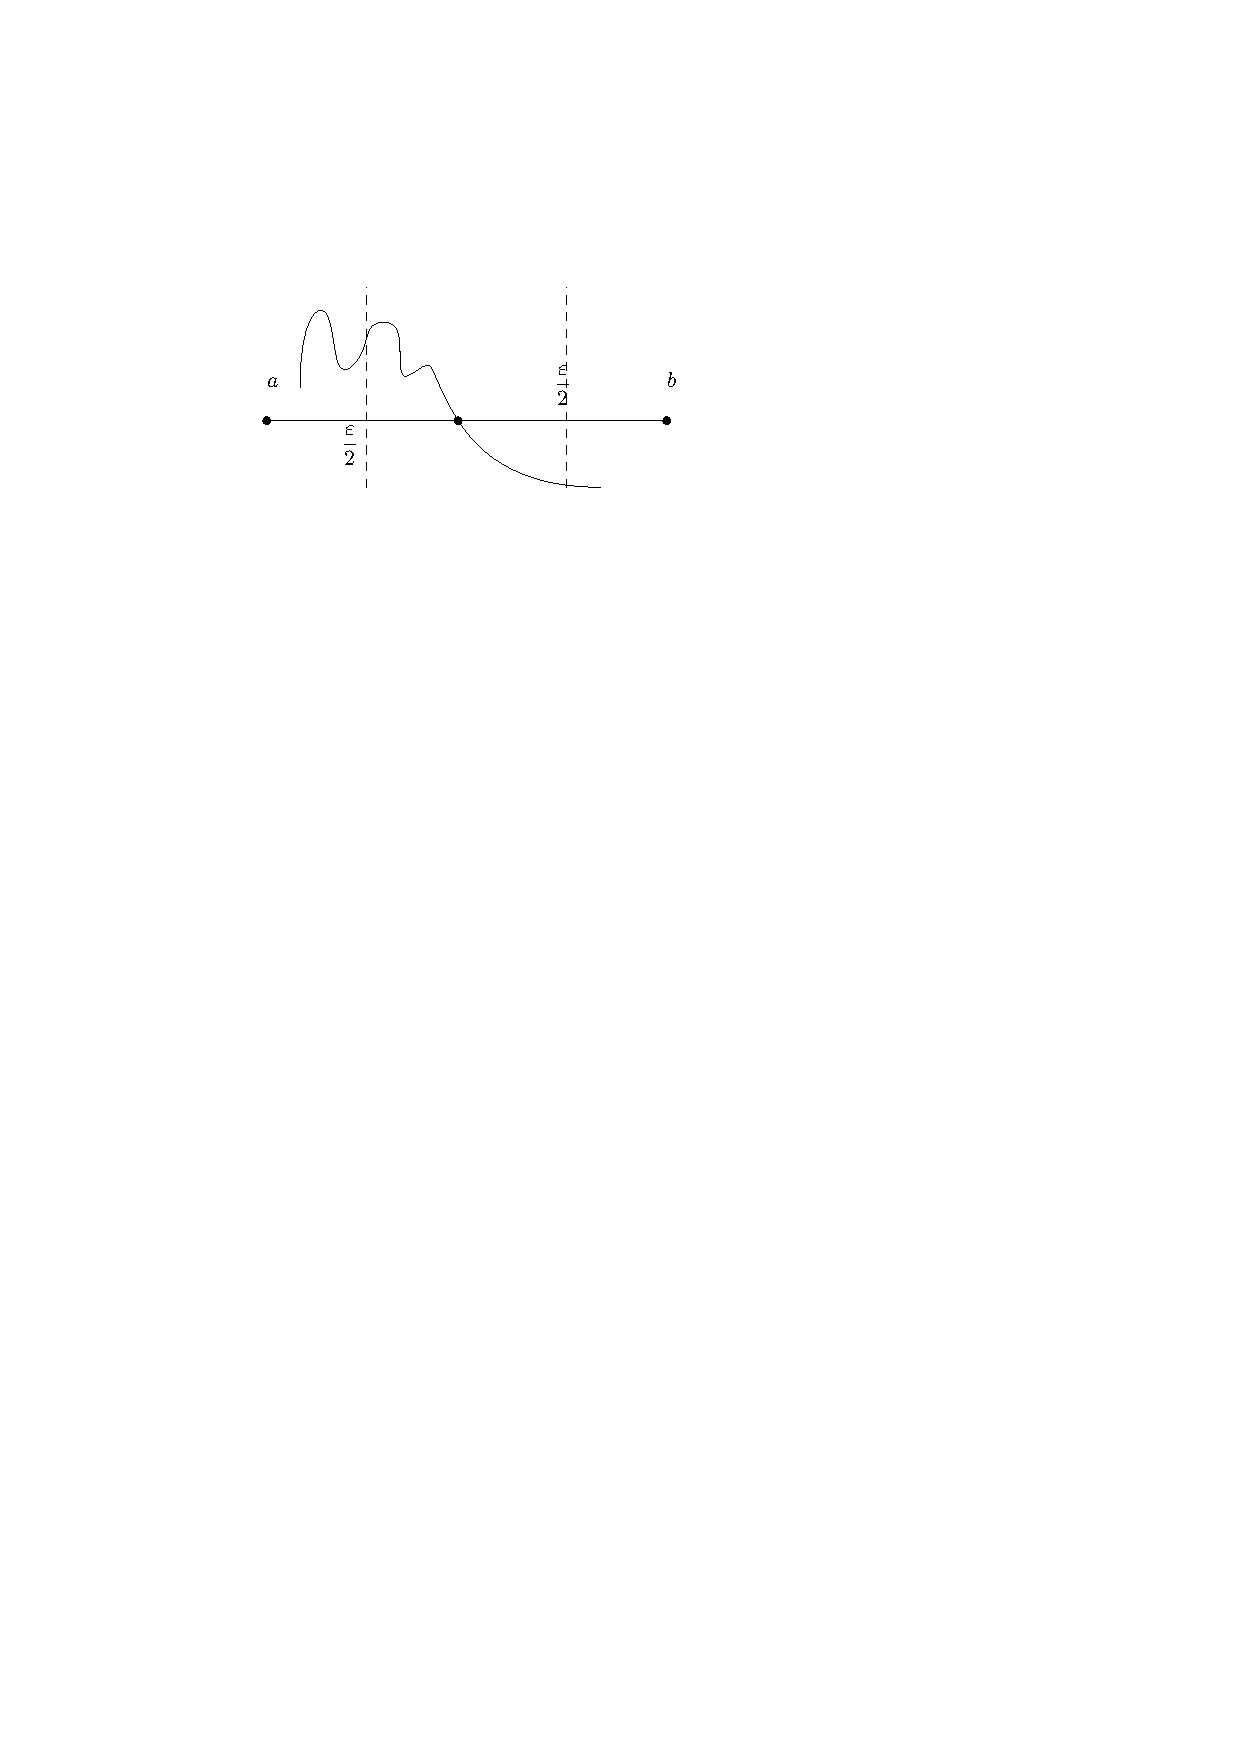
\includegraphics{image/自适应Simpson.pdf}
    \end{figure}
\end{note}
\subsection{二重积分计算方法}
\[
    \begin{aligned}
        I(f)&=\iint_{\Omega}f(x,y)dxdy\\
        & \int_a^b\mathrm{d}x\int_{\varphi(x)}^{\psi(x)}f(x,y)\mathrm{d}y = \int_{a}^{b}F(x)\mathrm{d}x \\
        & \approx\sum_{k = 0}^{n} A_{k}F(x_k)\\
        &\approx\sum_{k=0}^{n}A_{k}\left[\sum_{l=0}^{m}B_{kl}f(x_{k},y_{l})\right]
    \end{aligned}
\]

\begin{example}
    计算上述二重积分的梯形公式为
    \begin{solution}
        \[
            \begin{aligned}
                T(f)&=\frac{b-a}{2}[\frac{\psi(a)-\varphi(a)}{2}(f(a,\varphi(a))+f(a,\psi(a)))\\
                &+\frac{\psi(b)-\varphi(b)}{2}(f(b,\varphi(b))+f(b,\psi(b)))]
            \end{aligned}
        \]
    \end{solution}
\end{example}
\subsubsection{复合求积公式}
考虑矩形区域的重积分$\Omega=[a,b]\times[c,d]$
\[
    I(f)=\int_{a}^{b}\int_{c}^{d}f(x,y)\mathrm{d}x\mathrm{d}y
\]
\begin{note}
    复合梯形公式
    \[
        \begin{aligned}
            I(f)& =\iint_{\Omega}f(x,y)\mathrm{d}x\mathrm{d}y \\
            &\approx\frac{h_{x}h_{y}}{4}\sum_{i=0}^{n}\sum_{i=0}^{m}\lambda_{ij}f(x_{i},y_{j})
        \end{aligned}
    \]
    \[
        \Lambda=
        \begin{bmatrix}
            1&2&2&\cdots&2&2&1\\
            2&4&4&\cdots&4&4&2\\
            \vdots&\cdots&\vdots&\cdots&\cdots&\cdots\\
            2&4&4&\cdots&4&4&2\\
            1&2&2&\cdots&2&2&1
        \end{bmatrix}
        =(\lambda_{\mathbf{ij}})
    \]
\end{note}
\subsection{数值微分}
\subsubsection{机械求导公式}
\[
    f'(x_0) = \lim\limits_{h\to 0}\dfrac{f(x_0+h)-f(x_0)}{h}
\]
\[
    f'(x_0) \approx \dfrac{f(x_0+h)-f(x_0)}{h} = f'(x_0) + \dfrac{f''(x_0)}{2}h^2
\]
\begin{note}
    中点公式(二阶截断误差)
    \[
        G(h) = \dfrac{f(a+h)-f(a-h)}{2h}\quad \colorbox{cyan!50}{$h$过小,两相近的数相减,影响舍入误差}
    \]
    \[
        G(h) = f'(a) + \dfrac{h^2}{3!}f'''(a)+\dfrac{h^4}{5^!}f^{(5)}(a)+\cdots\quad \colorbox{red!50}{$h$小,截断误差小}
    \]
    \begin{itemize}
        \item \colorbox{cyan!50}{从舍入误差看,$h$不宜过小}
        \item \colorbox{red!50}{从截断误差看,$h$越小,计算越准确}
    \end{itemize}
\end{note}
\begin{example}
    以下关于数值微分的说法\colorbox{red!50}{不正确}的是 ()
    \begin{enumerate}
        \item[\choice{}{A}] 在实际应用中,基于插值多项式的微分方法,其插值次数不能太高
        \item[\choice{}{B}] 近似导数$f'(x)$的数值微分公式$\frac{f(x_{0}+h)-f(x_{0}-h)}{2h}$和$\frac{f(x_{0})-4f(x_{0}+h)+3f(x_{0}+2h)}{2h}$误差阶相同
        \item[\choice{}{C}] 数值微分公式的误差包括截断误差和舍入误差两部分
        \item[\choice{1}{D}] 当插值多项式$L_n(x)$收敛于$f(x)$时,其导数$L'_n(x)$收敛于$f'(x)$
    \end{enumerate}
\end{example}
\begin{definition}[插值型求导公式]
    建立$f(x)$的插值多项式$P_{n}(x)$,用$P'_{n}(x)$作为$f'(x)$的近似值
    \[
        f^{\prime}(x_{k})-P_{n}^{\prime}(x_{k})=\frac{f^{(n+1)}(\xi)}{(n+1)!}\omega_{n+1}^{\prime}(x_{k})
    \]
    其中$\omega_{n+1}^{\prime}(x_{k}) = (x-x_0)(x-x_1)(x-x_{k-1})\cdots(x-x_{k+1})(x-x_{n})$.

    两点公式:给定两个节点$x_0,x_1$,做线性插值多项式$P_{1}(x)$
    \[
        P_{1}^{\prime}(x_{0})=P_{1}^{\prime}(x_{1})=\frac{f(x_{1})-f(x_{0})}{h}
    \]
    \[
        f^{\prime}(x_{0})=P_{1}^{\prime}(x_{0})-\frac{h}{2}f^{\prime\prime}(\xi)\quad f^{\prime}(x_{1})=P_{1}^{\prime}(x_{1})+\frac{h}{2}f^{\prime\prime}(\xi)
    \]

    三点公式:给定三个节点$x_0,x_1,x_2$,做二次插值多项式$P_{2}(x)$
    \[
        P_{2}^{\prime}(x_{0})=\frac{-f(x_{2})+4f(x_{1})-3f(x_{0})}{2h}
    \]
    \[
        P_{2}^{\prime}(x_{1})=\frac{f(x_{2})-f(x_{0})}{2h}
    \]
    \[
        P_2'(x_2)=\frac{3f(x_2)-4f(x_1)+f(x_0)}{2h}
    \]
    以上公式近似相应导数的误差分别为$\frac{h^{2}}{3}f^{\prime\prime\prime}(\xi),-\frac{h^{2}}{6}f^{\prime\prime\prime}(\xi),\frac{h^{2}}{3}f^{\prime\prime\prime}(\xi).$
\end{definition}
